
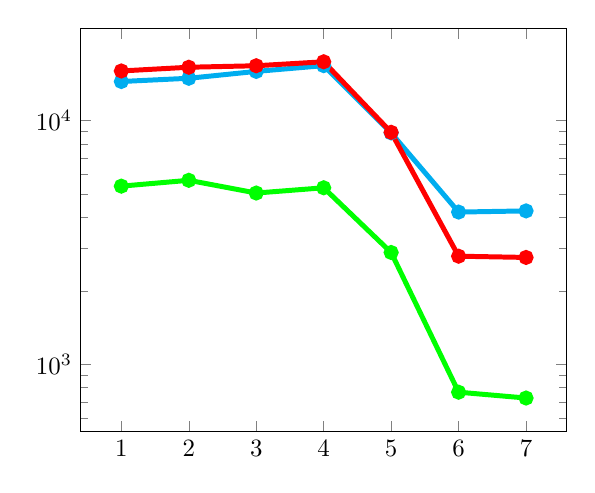
\begin{tikzpicture}[scale=0.9]
\begin{semilogyaxis}
\addplot[mark=*,color=cyan,line width=2pt,mark options={solid}] coordinates {(1,14466.302056)(2,14915.141763)(3,15915.937528)(4,16807.44934)(5,8897.951572)(6,4209.467145)(7,4256.189379)};
\addplot[mark=*,color=red,line width=2pt,mark options={solid}] coordinates {(1,15983.614369)(2,16555.489895)(3,16789.886104)(4,17433.006986)(5,8948.312123)(6,2773.313927)(7,2741.204448)};
\addplot[mark=*,color=green,line width=2pt,mark options={solid}] coordinates {(1,5378.403412)(2,5684.740647)(3,5039.525624)(4,5295.952172)(5,2872.894073)(6,766.722225)(7,725.489882)};

\end{semilogyaxis}
\end{tikzpicture}
